\documentclass[10pt]{article}
\usepackage[margin=0.85in]{geometry}
\usepackage{amsmath,amssymb,amsthm}
\usepackage[hidelinks]{hyperref}
\usepackage{tikz}
\usetikzlibrary{arrows.meta}

\newtheorem{theorem}{Theorem}
\newtheorem{lemma}[theorem]{Lemma}
\newtheorem{proposition}[theorem]{Proposition}
\newcommand{\pk}{\mathsf{pk}}
\newcommand{\sk}{\mathsf{sk}}
\newcommand{\Ent}{\mathsf{H}}
\newcommand{\KL}{\mathsf{D}}
\newcommand{\pos}[1]{\left[#1\right]_+}

\title{A Verification Lower Bound for Hash-Based One-Time Signatures}
\author{}
\date{}

\begin{document}
\maketitle

\begin{abstract}
A hash-based one-time signature reveals selected values of a fixed computation on secret inputs, and the verifier recomputes the final hash from these values and compares it with the public key. We ask how cheap this verification can be. The computation may combine hash queries with arbitrary deterministic operations, and we charge one hash unit for every 512 bits of hash input. For a 128-bit public key, signatures of at most 5504 bits, and a security requirement of roughly 127 bits against classical attackers, we prove that some signature must cost at least 25 hash units to verify. The proof is an explicit attack that turns one observed signature into a forgery on a new message. Its analysis bounds the information carried by the revealed values, counts the disclosure sets that this information leaves poorly protected, and bounds the cost of producing values that the verifier accepts for one of them.
\end{abstract}

\setcounter{tocdepth}{2}
\tableofcontents

\section{Introduction}\label{sec:intro}

A hash-based one-time signature scheme starts from a public computation on secret random inputs. Key generation runs the computation and publishes part of its final hash as the public key. To sign, the signer reveals the values of certain intermediate nodes, chosen according to the message. To verify, one recomputes the final hash from the revealed values and compares it with the public key. Lamport and Winternitz signatures follow this pattern. The model of Section~\ref{sec:model} covers them and any other scheme whose signatures consist of node values of a fixed computation, with the revealed nodes selected by hashing the message together with a nonce.

Three quantities compete in such a scheme: the length of the public key, the length of the signature, and the amount of hashing that verification requires. This note fixes the first two and asks for the least possible value of the third. We work in the random-oracle model and charge one \emph{hash unit} for every 512 bits of input hashed, so that a short input costs one unit and a long input costs proportionally more. Deterministic operations, such as splitting, concatenating, or otherwise transforming strings, are free, and the computation may use them without restriction. Our parameters are a 128-bit public key, signatures of at most 5504 bits, and a security requirement of roughly 127 bits: a classical attacker spending $B$ hash units must forge with probability below $B/2^{127}$.

\paragraph{Result.}
Under these constraints, some signature requires at least 25 hash units to verify (Theorem~\ref{thm:main}). One of these units pays for hashing the message together with a nonce, which selects the values to reveal; the remaining 24 are recomputation. In the other direction, Section~\ref{sec:scheme} gives a concrete scheme, a forest of hash chains under a small tree, whose signatures all verify in 106 units, and proves it secure (Theorem~\ref{thm:scheme}).

\paragraph{Proof idea.}
Suppose instead that every signature verifies within 24 units. Then recomputing the root from any signature evaluates at most 22 hash nodes besides the root. We exhibit an attacker that requests one signature and forges another.

The starting point is that a signature reveals at most 5248 bits, and these bits carry at most about 5248 bits of information about the signer's secret record, however the computation is arranged. We make this precise by assigning each hash node a \emph{weight}: the number of bits of its output that the revealed values pin down, once the secret inputs and the earlier outputs are given. The weights sum to at most 5257 bits, except with small probability (Lemma~\ref{lem:information}).

To forge with another set of revealed nodes, the attacker must supply values from which the verifier recomputes the same root. It samples a secret record consistent with everything it has seen and tests, at each hash node that the verifier will newly evaluate, whether the oracle agrees with the sampled record. Lemma~\ref{lem:conversion} shows that $q$ attempts succeed with probability at least $1-d/\log(eq\ln q)$ when the newly evaluated nodes have total weight $d$. A target of weight $d$ is therefore reached after somewhat fewer than $2^d$ attempts.

A scheme would like every other target set to be expensive. But there are $2^{115}$ sets, each touching at most 22 hash nodes, and only about 5257 bits of weight to distribute among them. A counting argument (Lemma~\ref{lem:counting}) shows that the observed signature typically leaves dozens of sets of weight below 123 bits, and about $2^{115}$ construction attempts suffice for a set of that weight. It remains to select a cheap set for the new message. The set is chosen by hashing the message with a nonce, and the attacker searches for a nonce landing on one of the hundred lowest-weight sets. These form a $100/2^{128}$ fraction of the possible hash values, so about $2^{121}$ nonce trials suffice. The total cost is about $2^{123}$ units, and the attack succeeds with probability above one in twenty. The ratio of cost to success probability falls below $2^{127}$, contradicting the security requirement. The margin is small, so the final comparisons are carried out in exact rational arithmetic (Appendix~\ref{sec:numerical}).

\paragraph{Organization.}
Section~\ref{sec:model} defines the model and states the theorem. Section~\ref{sec:information} defines the weights and proves the information bound. Section~\ref{sec:conversion} constructs values for a target set and bounds the cost of doing so. Section~\ref{sec:counting} proves the counting bound. Section~\ref{sec:attack} assembles the attack and completes the proof. Section~\ref{sec:scheme} describes a concrete scheme and proves its security. Appendix~\ref{sec:elementary} collects elementary facts about entropy and repeated trials, and Appendix~\ref{sec:numerical} verifies the numerical inequalities.

\section{Model and result}\label{sec:model}

Key generation evaluates a public computation on random secret inputs. A signature reveals values at selected nodes of this computation. These values must suffice to recompute its final hash, whose first 128 bits the verifier compares with the public key. We specify the computation, the choice of revealed nodes, and the security requirement below.

\subsection{The computation and its cost}

We model hashing by a random oracle $H$. A query consists of a public label $\tau$ and a nonempty bit string $u$. For each distinct pair $(\tau,u)$, the oracle assigns an independent, uniformly random 256-bit answer $H(\tau,u)$. Repeating a query returns the same answer. The cost of a query with input $u$ is
\[
c(u)=\left\lceil\frac{|u|}{512}\right\rceil
\]
hash units. The label does not contribute to the cost. All other computation, storage, and private randomness are free, for both the signer and the attacker.

The computation is a finite directed acyclic graph (DAG). An edge from $v$ to $w$ means that $w$ uses the value of $v$. Each node $v$ has a fixed output length $b_v$. There are three types of nodes:
\begin{description}
\item[Secret sources.] A source has no parents and holds a uniformly random string of its prescribed length. All source strings are independent.
\item[Deterministic nodes.] A deterministic node applies a public, oracle-free function to its parents' values in a specified order. Such a function may concatenate strings, select bits, or perform any other deterministic computation. A deterministic node with no parents outputs a public constant.
\item[Hash nodes.] A hash node has one parent and a public label. It queries $H$ on that label and its parent's value. Its output has length 256, and its parent's output length is positive. Different hash nodes have different labels.
\end{description}
The graph has a unique node with no outgoing edges, called the root. The root is a hash node, and every other node has a directed path to it. The graph, functions, lengths, labels, and parent orders are public and fixed independently of the oracle.

Key generation samples the source strings and evaluates the graph in a fixed topological order, with parents before children. Number the hash nodes $1,\ldots,n$ in this order; the root is $r=n$. At hash node $g$, denote the label by $\tau_g$, the input by $I_g$, and the output by $Y_g=H(\tau_g,I_g)$. The cost $c_g=c(I_g)$ is fixed because the input length is fixed.

Let $Z$ be the tuple of source strings. The signer stores the \emph{secret record}
\[
\sk=(Z,Y_1,\ldots,Y_n).
\]
The source strings and stored hash outputs determine every deterministic node value without further oracle queries. The public key $\pk$ is the first 128 bits of $Y_r$. Key generation costs $\sum_{g=1}^n c_g$ units.

\subsection{Reconstructing the root from revealed values}

Write $X_v$ for the value of node $v$ during key generation. For a node set $A$, let $X_A=(X_v)_{v\in A}$, with entries listed in a fixed public order.

The scheme specifies $M$ sets $A_0,\ldots,A_{M-1}$ of nodes whose values may be revealed. We call these the \emph{disclosure sets}; $i$ is their index, and $X_{A_i}$ is the tuple of values revealed at index $i$. Every $A_i$ excludes the root and intersects every directed path from a secret source to the root. The first condition forces the verifier to recompute the root rather than receive it. The second guarantees that the revealed values suffice for this recomputation, as shown below. The sets are fixed independently of the oracle. The tuple for index $i$ occupies
\[
\ell_i=\sum_{v\in A_i}b_v
\]
bits. Its entries have known lengths and order, so the signature need not include node identifiers or delimiters.

Root reconstruction takes an index $i$ and a string $x$ of length $\ell_i$. Split $x$ into values for the nodes of $A_i$. Starting at the root, follow edges backward and stop whenever a node in $A_i$ is reached. Evaluate the remaining visited nodes in topological order, using the supplied values at the stopping nodes. Store each computed value for reuse.

This procedure needs no secret inputs beyond those supplied in $x$. If the backward traversal reached an undisclosed secret source, it would give a source-to-root path missing $A_i$, contrary to the path condition. Every other visited node is either a public constant or can be evaluated from its parents. The root itself is evaluated because it does not belong to $A_i$.

Let $E_i$ be the set of hash nodes evaluated by this procedure. It is determined by the graph and the set $A_i$, not by the string $x$. Each node in $E_i$ is evaluated once, so reconstruction costs $\sum_{g\in E_i}c_g$ units.

If the supplied string $x$ contains the values computed at the nodes of $A_i$ during key generation, reconstruction produces the same root output as key generation. This follows by induction in evaluation order. The supplied values are the original node values. Each deterministic node therefore receives its original inputs, and each hash node makes its original oracle query. Hence every reconstructed value agrees with key generation, including the root output $Y_r$. This holds for every source assignment and every oracle.

\subsection{Signatures and security}

For a 256-bit message $m$ and a 256-bit nonce $\eta$, let $\mathsf{idx}(m,\eta)$ be the integer represented by the first 128 bits of $H(\tau_{\mathrm{enc}},m\Vert\eta)$, where $\Vert$ denotes concatenation. The label $\tau_{\mathrm{enc}}$ is reserved for this query and differs from every hash-node label. Computing $\mathsf{idx}$ costs one unit.

To sign $m$, choose $\eta$ uniformly from the nonces not yet tried in this signing call and compute $i=\mathsf{idx}(m,\eta)$. If $i<M$, return the signature $(\eta,X_{A_i})$. Otherwise, try another nonce. Signing fails after $L$ unsuccessful trials.

To verify $(\eta,x)$ on message $m$, first check that $\eta$ has 256 bits. Compute $i=\mathsf{idx}(m,\eta)$ and reject if $i\ge M$ or $|x|\ne\ell_i$. Otherwise, reconstruct the root from $(i,x)$ and accept if the first 128 bits of the result equal $\pk$. Thus, for a signature selecting index $i$, the length and verification cost are
\[
|\sigma|=256+\ell_i,
\qquad
C_i=1+\sum_{g\in E_i}c_g.
\]
We require $\ell_i\le S$ for every $i$ and $\sum_g c_g\le K$, with parameters
\[
\begin{array}{lr}
\text{Public-key length} & 128\text{ bits}\\
\text{Message and nonce lengths} & 256\text{ bits each}\\
\text{Maximum signature length }256+S & 5504\text{ bits}\\
\text{Key-generation budget }K & 1024\text{ units}\\
\text{Number of disclosure sets }M & 2^{115}\\
\text{Signing trial limit }L & 2^{21}.
\end{array}
\]
After the 256-bit nonce, a signature therefore has $S=5248$ bits for revealed values. Since $\mathsf{idx}$ is a uniform 128-bit value, a signing trial selects a valid index with probability $M/2^{128}=2^{-13}$, and the trial limit $L$ makes signing failure negligible; see~\eqref{eq:abort}.

An attacker receives $\pk$, can query $H$, and may request one signature on a message of its choice. A forgery is a message--signature pair accepted by the verifier that differs from the pair returned by the signer. If no signature is returned, any accepted pair counts as a forgery. For every classical attacker whose total cost is at most $B$ in every execution, we require
\begin{equation}\label{eq:security}
\Pr[\mathrm{Forge}]<\frac{B}{2^{127}}.
\end{equation}
The probability is over the oracle, the source strings, and all signing and attack randomness. The cost includes key generation, signing, the attacker's queries, and final verification. Only oracle queries are charged; there is no bound on the attacker's other computation. Informally, the requirement says that a forgery costs about $2^{127}$ hash units per unit of success probability.

\begin{theorem}\label{thm:main}
In the model of this section, with the parameters listed above, every scheme satisfying the security requirement~\eqref{eq:security} has
\[
\max_{0\le i<M}C_i\ge25.
\]
\end{theorem}

The proof occupies the rest of the paper. We assume instead that every $C_i\le24$ and construct an attacker that violates~\eqref{eq:security}. The attacker requests a signature on a message $m_1$ and then builds a signature on a different message $m_2$. Section~\ref{sec:information} describes the secret records consistent with the observed signature and bounds the information it reveals. Section~\ref{sec:conversion} shows how to produce values for another disclosure set and bounds the cost. Section~\ref{sec:counting} shows that many disclosure sets are cheap in this sense. Section~\ref{sec:attack} analyzes the nonce search that selects one of them and adds up costs and probabilities.

\section{Information in the revealed values}\label{sec:information}

We begin with the information obtained at a fixed index $i$: the honest values $X_{A_i}$ and the hash answers computed when reconstructing the root from them. Throughout this section and the next two, the index is fixed independently of key generation. Section~\ref{sec:attack} shows that the index selected by signing has this property, so the analysis applies to it.

\subsection{Records consistent with the observations}

Each hash node uses a distinct oracle label. Its query during key generation therefore receives a uniform 256-bit answer independent of the source strings and all earlier hash answers. Consequently, $Z,Y_1,\ldots,Y_n$ are mutually independent and uniform before any values are revealed.

To describe possible secret records, consider an arbitrary assignment
\[
\xi=(z,y_1,\ldots,y_n)
\]
of source strings and hash outputs of the prescribed lengths. Evaluate the deterministic nodes using $z$ at the sources and the stored value $y_g$ at hash node $g$, without querying $H$. Denote the resulting value at node $v$ by $X_v(\xi)$, and the resulting input to hash node $g$ by $I_g(\xi)$. In particular, $X_g(\xi)=y_g$ at a hash node. Write $X_A(\xi)$ for the tuple on a node set $A$. For the actual secret record, $X_v(\sk)=X_v$ and $I_g(\sk)=I_g$.

This evaluation is defined even if some stored output $y_g$ differs from the real answer $H(\tau_g,I_g(\xi))$. Every assignment $\xi$ is consistent with some oracle: prescribe the answer $y_g$ at $(\tau_g,I_g(\xi))$ for each $g$. The distinct labels ensure that these prescriptions never conflict.

Let $x$ be the honest values revealed at $A_i$. Reconstruct the root from $(i,x)$ using the real oracle, and let $y=(y_g)_{g\in E_i}$ be the hash answers obtained, listed in node order. Since computation is free, the attacker can enumerate the set
\[
\mathcal C
=\{\xi:X_{A_i}(\xi)=x
\text{ and }X_g(\xi)=y_g\text{ for every }g\in E_i\}.
\]
Its elements are the \emph{candidate records}. The actual secret record belongs to $\mathcal C$.

Every candidate agrees with the real oracle at the queries made during reconstruction from $(i,x)$. To see this, take a candidate $\xi$ and compare its node values with those computed during reconstruction, in evaluation order. The supplied values at $A_i$ agree with $\xi$ by definition of the candidate set. At a deterministic node, matching parent values give matching outputs. At each hash node $g$ evaluated during reconstruction, that is, each $g\in E_i$, the parent value gives the input $I_g(\xi)$. The real oracle's recorded answer at this node is $y_g$, which equals the candidate's stored output $X_g(\xi)$. Induction therefore gives
\[
H(\tau_g,I_g(\xi))=X_g(\xi)
\qquad(g\in E_i,\ \xi\in\mathcal C).
\]
No such agreement is asserted for hash nodes outside $E_i$.

Define $Q$ to be the probability distribution obtained by choosing one record uniformly from the candidate set $\mathcal C$. Explicitly, for each possible record $\xi$,
\[
Q(\xi)=
\begin{cases}
1/|\mathcal C|,&\xi\in\mathcal C,\\
0,&\xi\notin\mathcal C.
\end{cases}
\]
Here $|\mathcal C|$ is the number of candidates. The set is nonempty because it contains the actual secret record. Both $\mathcal C$ and $Q$ depend on the index $i$ and the observed values $x,y$; these are kept fixed when sampling from $Q$. To sample, the attacker enumerates $\mathcal C$ and chooses one of its records with equal probability, without making further oracle queries.

This distribution also describes the actual secret record conditional on the observations $x,y$. Before these values were observed, all records were equally likely. The observations exclude exactly the records outside $\mathcal C$, so the records inside $\mathcal C$ remain equally likely.

Probabilities written $\Pr_Q$ refer to choosing a candidate according to $Q$. For example, $\Pr_Q[Y_g=b]$ is the fraction of candidates whose stored output at hash node $g$ equals $b$. Likewise, $Z$ denotes the source strings in the chosen candidate. Sampling from $Q$ does not generate a new oracle or guarantee agreement with its unqueried entries.

\subsection{An information bound}

We assign a nonnegative weight to each hash node. The weight measures how much the revealed values constrain its output, once the source strings and earlier outputs are specified. Section~\ref{sec:conversion} will relate the sum of these weights to the probability of constructing values that pass the root check.

All logarithms are base two unless written $\ln$. Let $U,V$ be quantities determined by a candidate record sampled from $Q$. Write $Q(u,v)=\Pr_Q[U=u,V=v]$ for their joint probabilities and $Q(u\mid v)=\Pr_Q[U=u\mid V=v]$ for their conditional probabilities. The \emph{conditional Shannon entropy} of $U$ given $V$, measured in bits, is
\[
\Ent_Q(U\mid V)
=\sum_{u,v:Q(u,v)>0}Q(u,v)\log\frac1{Q(u\mid v)},
\]
which measures the average uncertainty in $U$ after $V$ is specified. The same definition applies to other finite probability distributions. Omit the conditioning variable to write $\Ent_Q(U)$, and omit the subscript when the distribution is clear. A uniform 256-bit string has entropy 256; every 256-bit string has entropy at most 256. The required entropy identities are proved in Appendix~\ref{sec:elementary}.

Write $Y_{<g}=(Y_1,\ldots,Y_{g-1})$, with an empty tuple when $g=1$. Define
\begin{equation}\label{eq:weights}
h_i(g)=
\begin{cases}
256-\Ent_Q(Y_g\mid Z,Y_{<g}),&g\notin E_i,\\
0,&g\in E_i.
\end{cases}
\end{equation}
Before the observations, $Y_g$ is independent of $Z,Y_{<g}$ and has entropy 256. The first line measures the reduction in that entropy among candidate records. Nodes in $E_i$ receive weight zero because their input--output pairs have already been checked. Conditioning on $Z,Y_{<g}$ is part of the analysis; it does not assume that the attacker knows these values. Although denoted by $h_i$, the weights depend on both observed tuples $x,y$. For a set $A$ of hash nodes, put $h_i(A)=\sum_{g\in A}h_i(g)$.

The total weight is unlikely to exceed the number of revealed bits by much.

\begin{lemma}[Information bound]\label{lem:information}
For a fixed index $i$ and every $u\ge0$,
\[
\Pr\left[\sum_{g=1}^n h_i(g)>\ell_i+u\right]\le2^{-u}.
\]
The probability is over key generation and the resulting observations. In particular, with
\[
S_*=S+9=5257,\qquad \varepsilon=2^{-9},
\]
the total weight is at most $S_*$ except with probability at most $\varepsilon$.
\end{lemma}

\begin{proof}
We first show that a large total weight is possible only when few secret records give the revealed values. We then bound the probability of observing such values.

Fix the answers $y$ at the reconstructed hash nodes, but do not yet specify the revealed tuple $x$. Let $b_{\mathrm{src}}$ be the total length of the source strings. There are
\[
N_y=2^{b_{\mathrm{src}}+256(n-|E_i|)}
\]
records with these answers: the source strings and the $n-|E_i|$ other hash outputs can be chosen freely. These records are equally likely, by their independence and uniformity.

Now specify a possible revealed tuple $x$. Its candidate set $\mathcal C$ consists of the records among these $N_y$ that give $x$. Thus, conditional on the answers $y$, the probability of observing $x$ is $|\mathcal C|/N_y$.

The distribution $Q$ is uniform on these candidates, so the Shannon entropy of the complete record is $\Ent_Q(\sk)=\log|\mathcal C|$. The entropy chain rule writes this as the uncertainty in the sources followed by that in each successive hash output:
\[
\log|\mathcal C|
=\Ent_Q(Z)+\sum_{g\notin E_i}\Ent_Q(Y_g\mid Z,Y_{<g}).
\]
Outputs in $E_i$ contribute zero because their values are already fixed to $y$. The sources contain $b_{\mathrm{src}}$ bits, so $\Ent_Q(Z)\le b_{\mathrm{src}}$. Using the definition of the weights, we obtain
\begin{equation}\label{eq:entropy-budget}
\begin{aligned}
\sum_g h_i(g)
&=256(n-|E_i|)-\log|\mathcal C|+\Ent_Q(Z)\\
&\le256(n-|E_i|)+b_{\mathrm{src}}-\log|\mathcal C|\\
&=\log\frac{N_y}{|\mathcal C|}.
\end{aligned}
\end{equation}
The entropy facts used here are proved in Appendix~\ref{sec:elementary}.

If the total weight exceeds $\ell_i+u$, this bound forces $|\mathcal C|/N_y<2^{-\ell_i-u}$. In other words, the observed tuple $x$ must have conditional probability below $2^{-\ell_i-u}$. There are at most $2^{\ell_i}$ tuples of length $\ell_i$. Adding the probabilities of all tuples below this threshold gives at most $2^{\ell_i}2^{-\ell_i-u}=2^{-u}$. This bound holds for every choice of $y$, so it also holds after averaging over the reconstructed answers.
\end{proof}

\section{Producing values for a target set}\label{sec:conversion}

The attacker has received the values $x$ at the nodes of $A_i$ and recorded the hash answers $y$ while reconstructing the root. It has therefore formed the candidate set $\mathcal C$. We now explain how to use these candidates to produce values for a chosen target set $A_j$.

The task is to find a string $x'$ such that reconstruction from $(j,x')$ returns the original root output $Y_r$. This is only the node-value part of a signature. Later, the attacker will search for a nonce $\eta'$ selecting $j$ on a new message $m_2$. Together, that nonce and $x'$ will form the forgery.

If we use a candidate's values at $A_j$, reconstruction will evaluate the hash nodes in $E_j$. At nodes also belonging to $E_i$, the candidate's input--output pairs already agree with the real oracle, as proved in Section~\ref{sec:information}. Our construction checks the remaining nodes,
\[
J=E_j\setminus E_i.
\]

\subsection{One construction attempt}

Start with a working set containing all records in $\mathcal C$. Process the nodes $g\in J$ in topological order. At each node:
\begin{enumerate}
\item Sample a record $\xi$ uniformly from the working set and compute $u=I_g(\xi)$.
\item Query $H(\tau_g,u)$ and call the answer $v$.
\item Retain exactly the records $\xi'$ in the working set for which $I_g(\xi')=u$ and $X_g(\xi')=v$. If no record remains, stop and report failure.
\end{enumerate}
Sampling a record does not commit the attempt to using that record later. It only chooses the next query input. If all checks finish, choose any remaining record $\xi'$ and return $x'=X_{A_j}(\xi')$.

Computing node values from a record and filtering the working set require no oracle queries. Each attempt costs at most $\sum_{g\in J}c_g$ units.

To check correctness, consider a record $\xi'$ that survives all checks. For each $g\in E_j$, its pair $(I_g(\xi'),X_g(\xi'))$ agrees with the real oracle: this was observed initially if $g\in E_i$ and checked during the attempt otherwise. Now reconstruct the root from $(j,X_{A_j}(\xi'))$. The supplied values agree with $\xi'$. Inductively, each deterministic node computes its value under $\xi'$, and each hash node receives the input $I_g(\xi')$ and returns $X_g(\xi')$. The final output is $X_r(\xi')=y_r=Y_r$, since the root belongs to $E_i$ and every candidate stores its observed output.

\subsection{The probability of success}

The total weight of $J$ bounds the success probability of repeated attempts. The first part of the next lemma is a bound for one attempt; the second part turns it into a bound after repetition.

\begin{lemma}[Construction bound]\label{lem:conversion}
Fix the index $i$, the observed tuples $x,y$, and the target index $j$. Put $d=h_i(J)$. For a fixed oracle $H$, let $p(H)$ be the probability that one construction attempt finishes, over its private randomness. Then
\begin{equation}\label{eq:log-success}
\mathbb E_H[-\log p(H)]\le d,
\end{equation}
where the oracle is distributed conditional on $x,y$. For every integer $q\ge3$, at least one of $q$ attempts finishes with probability at least
\begin{equation}\label{eq:conversion}
\pos{1-\frac{d}{\log(e q\ln q)}},
\qquad [t]_+=\max\{t,0\}.
\end{equation}
Each attempt starts from the original candidate set and uses independent private randomness. Their total cost is at most $q\sum_{g\in J}c_g$.
\end{lemma}

\begin{proof}
If $J$ is empty, the attempt makes no queries and always finishes. Otherwise, list its nodes as $g_1,\ldots,g_m$ in topological order. All probabilities and entropies in this proof are conditional on the fixed observations $x,y$. Under this conditioning, the actual secret record has distribution $Q$.

Let
\[
\mathcal T=((I_{g_1},Y_{g_1}),\ldots,(I_{g_m},Y_{g_m}))
\]
be the sequence of input--output pairs at these nodes in the actual secret record. Call this sequence a \emph{trace}, and write $\mathcal T_{<k}$ for its first $k-1$ pairs. The proof compares this trace with the sequence of queries and answers in a successful attempt.

\paragraph{Information about the trace contained in the oracle.}
Only finitely many oracle entries can be queried during an attempt: those at the labels $\tau_g$ for $g\in J$, with the input length prescribed for each node. Let $\mathcal O$ be the collection of these entries and $N_J$ their number. Each entry has 256 bits, so
\[
\Ent(\mathcal O)\le256N_J.
\]

Given a complete secret record, one entry in each of these tables is fixed: $H(\tau_g,I_g)$ must equal $Y_g$. The observations $x,y$ are determined by that record and impose no further conditions once it is fixed. The other entries remain independent and uniform, because key generation queried no other input at these labels. Every record with a given trace fixes exactly the same entries. Therefore, conditioning only on the trace still leaves all other entries independent and uniform, and
\[
\Ent(\mathcal O\mid\mathcal T)=256(N_J-m).
\]
The entropy chain rule now gives
\begin{equation}\label{eq:oracle-entropy}
\Ent(\mathcal T\mid\mathcal O)
=\Ent(\mathcal T)+\Ent(\mathcal O\mid\mathcal T)-\Ent(\mathcal O)
\ge\Ent(\mathcal T)-256m.
\end{equation}
Thus learning these oracle tables reduces uncertainty about the actual trace by at most 256 bits per node in $J$.

\paragraph{Comparing actual traces with successful attempts.}
For a trace $t=((u_1,v_1),\ldots,(u_m,v_m))$ that occurs under $Q$, define
\[
a(t)=\prod_{k=1}^m
\Pr_Q[I_{g_k}=u_k\mid\mathcal T_{<k}=t_{<k}].
\]
After the first $k-1$ checks follow $t_{<k}$, the working set is exactly the set of candidates with these pairs. Its next uniform sample therefore chooses the input $u_k$ with the probability in the $k$th factor.

Fix a value $o$ of the oracle tables with positive conditional probability. The attempt depends on $H$ only through these tables, so write $p(o)$ for its success probability. Define
\[
\mu_o(t)=\Pr[\mathcal T=t\mid\mathcal O=o].
\]
If $\mu_o(t)>0$, the trace occurs in a candidate and agrees with the tables $o$. The attempt follows it with probability $a(t)>0$: each chosen input receives the specified answer, and that candidate survives every check. Hence $p(o)>0$.

Let $\nu_o$ be the distribution of the attempt's trace conditional on success with tables $o$. On every trace with $\mu_o(t)>0$, we have $\nu_o(t)=a(t)/p(o)$. We compare these distributions using their relative entropy. For distributions $R,S$ on a finite set, this is $\KL(R\Vert S)=\sum_{t:R(t)>0}R(t)\log(R(t)/S(t))$, with value infinity if $S(t)=0<R(t)$ anywhere. It is nonnegative, as proved in Appendix~\ref{sec:elementary}. Applying this fact gives
\[
\begin{aligned}
0
&\le\KL(\mu_o\Vert\nu_o)\\
&=\sum_{t:\mu_o(t)>0}\mu_o(t)\log\frac{\mu_o(t)p(o)}{a(t)}\\
&=-\Ent(\mathcal T\mid\mathcal O=o)-\mathbb E[\log a(\mathcal T)\mid\mathcal O=o]+\log p(o).
\end{aligned}
\]
Rearrange and average over $\mathcal O$:
\[
\mathbb E[-\log p(\mathcal O)]
\le-\mathbb E[\log a(\mathcal T)]-\Ent(\mathcal T\mid\mathcal O).
\]
By the definition of $a$,
\[
-\mathbb E[\log a(\mathcal T)]
=\sum_{k=1}^m\Ent_Q(I_{g_k}\mid\mathcal T_{<k}).
\]
Using~\eqref{eq:oracle-entropy} and expanding the entropy of the trace into successive inputs and outputs, we obtain
\begin{equation}\label{eq:conversion-entropy}
\begin{aligned}
\mathbb E[-\log p(\mathcal O)]
&\le\sum_{k=1}^m\Ent_Q(I_{g_k}\mid\mathcal T_{<k})-\Ent_Q(\mathcal T)+256m\\
&=\sum_{k=1}^m\bigl(256-\Ent_Q(Y_{g_k}\mid\mathcal T_{<k},I_{g_k})\bigr)\\
&\le\sum_{k=1}^m h_i(g_k)=d.
\end{aligned}
\end{equation}
The final inequality follows because $Z,Y_{<g_k}$ determine both $\mathcal T_{<k}$ and $I_{g_k}$. Conditioning on the source strings and all earlier outputs therefore gives at least as much information as conditioning on these earlier pairs and the current input. In particular,
\[
\Ent_Q(Y_{g_k}\mid\mathcal T_{<k},I_{g_k})
\ge\Ent_Q(Y_{g_k}\mid Z,Y_{<g_k}).
\]
Since $p(H)$ depends only on $\mathcal O$, this proves~\eqref{eq:log-success}.

\paragraph{Repetition.}
For a fixed oracle, the attempts use the same initial set $\mathcal C$ and independent randomness. Their common success probability is $p(H)$, even if they repeat oracle queries. All $q$ fail with probability $(1-p(H))^q$. Lemma~\ref{lem:repetition} proves
\[
(1-p)^q\le\frac{-\ln p}{\ln q+\ln\ln q+1}
\qquad(q\ge3,\ 0<p\le1).
\]
Averaging this inequality over the oracle and applying~\eqref{eq:log-success} bounds the probability of failure by $d/\log(e q\ln q)$. This gives~\eqref{eq:conversion}.
\end{proof}

\section{Counting low-weight targets}\label{sec:counting}

A low value of $h_i(E_j\setminus E_i)$ gives a useful construction bound for target index $j$. The nonce search will need many such indices. We now show that most observations leave many targets of low weight.

For each index $j$, define $V_j=E_j\setminus\{r\}$. This is the set of hash nodes other than the root evaluated during reconstruction at $j$. Since the root belongs to $E_i$ and $h_i$ vanishes on $E_i$,
\[
h_i(E_j\setminus E_i)=h_i(V_j).
\]
The counting argument uses only the size of each $V_j$, the fact that $h_i$ vanishes on $V_i$, and a bound on the total weight. We state it for an arbitrary finite collection of weighted sets. The idea is to order the underlying elements at random and to look, for each set, at the position where its last element appears. Every set completed before $V_i$ lies inside the initial segment ending at $V_i$. If that segment carries little weight under $h_i$, all of these sets are low-weight targets for $i$, and the nesting of initial segments limits how many indices can have few such targets.

\begin{lemma}[Counting bound]\label{lem:counting}
Let $V_0,\ldots,V_{M-1}$ be subsets of a finite set $\mathcal U$, each of size at most an integer $a\ge1$. For each $i$, let $h_i:\mathcal U\to[0,\infty)$ be a weight function that is zero on $V_i$, and write $h_i(A)=\sum_{g\in A}h_i(g)$. For a fixed bound $S_*>0$, call $i$ \emph{good} when $\sum_{g\in\mathcal U}h_i(g)\le S_*$.

For a threshold $d>0$, define
\begin{equation}\label{eq:beta}
\rho=\frac{S_*}{d},
\qquad
\beta_a(d)=\prod_{k=1}^{a}
\frac{(a-1)\rho/(1+\rho)+k}{a\rho+k}.
\end{equation}
For every integer $R\ge1$, the number of good indices $i$ for which
\[
\bigl|\{j:h_i(V_j)<d\}\bigr|<R
\]
is at most $(R-1)/\beta_a(d)$. Indices $j$ are counted separately even when their sets $V_j$ coincide.
\end{lemma}

\begin{proof}
Enlarge each $V_i$ to size exactly $a$ by adding new elements, different for each set. Give these elements weight zero under every $h_i$. None of the quantities $h_i(V_j)$ changes. From now on, $\mathcal U$ includes the added elements.

Choose a uniformly random ordering of $\mathcal U$. Let $P_i$ be the set of elements up to and including the last element of $V_i$ in this order. Thus the sets $P_i$ are nested: for any two, one contains the other. For each good index $i$, we will find an event $U_i$ with probability at least $\beta_a(d)$ on which every set $V_j\subseteq P_i$ has weight $h_i(V_j)<d$. The nesting will then bound the number of good indices with few low-weight targets.

\paragraph{Reducing to a bounded number of positive weights.}
Fix a good index $i$. We first reduce the number of positive weights by subtracting a common amount, without letting any weight become negative. Put $n_0=\lfloor a\rho\rfloor$. Let $\alpha$ be the $(n_0+1)$st largest weight under $h_i$, counting repetitions, or zero if $|\mathcal U|<n_0+1$. Define the reduced weights and threshold by
\[
w_g=\max\{h_i(g)-\alpha,0\},
\qquad
b=d-a\alpha.
\]
At most $n_0$ original weights exceed $\alpha$, so at most $n_0$ reduced weights are positive. Since $(n_0+1)\alpha\le S_*$ and $n_0+1>aS_*/d$, we have $a\alpha<d$ and hence $b>0$. The reduction removes at least $(n_0+1)\alpha$ in total: when $\alpha>0$, at least $n_0+1$ elements lose exactly $\alpha$, and when $\alpha=0$ the claim is immediate. Thus
\[
\sum_g w_g\le S_*-(n_0+1)\alpha
\le\rho(d-a\alpha)=\rho b.
\]
For every element, $h_i(g)\le\alpha+w_g$. Since each $V_j$ has $a$ elements,
\[
h_i(V_j)\le a\alpha+\sum_{g\in V_j}w_g.
\]
In particular, on the event
\[
U_i=\left\{\sum_{g\in P_i}w_g<b\right\},
\]
every $V_j\subseteq P_i$ satisfies $h_i(V_j)<a\alpha+b=d$. It remains to bound $\Pr[U_i]$.

\paragraph{Bounding the probability of $U_i$.}
Let $n\le a\rho$ be the number of elements with positive reduced weight, and let $s=\sum_g w_g\le\rho b$. First order just these $n$ elements uniformly at random. Add their weights in that order. Let $X$ be the number of elements strictly before the partial sum first reaches or exceeds $b$. If the total is less than $b$, set $X=n$.

We claim that
\begin{equation}\label{eq:stopping}
\mathbb E(X+1)\ge\frac{(n+1)b}{s+b}.
\end{equation}
We prove this for arbitrary nonnegative weights and positive $b$, by induction on $n$. When $n=0$, both sides equal one. For $n>0$, temporarily number the elements $1,\ldots,n$ and condition on the first element $j$. If $w_j\ge b$, then $X=0$. If $w_j<b$, the remaining problem has $n-1$ elements, total weight $s-w_j$, and threshold $b-w_j$. Its induction bound is $n(b-w_j)/(s+b-2w_j)$. Averaging over the $n$ equally likely first elements gives
\[
\begin{aligned}
\mathbb E(X+1)
&\ge1+\sum_{j:w_j<b}\frac{b-w_j}{s+b-2w_j}\\
&\ge1+\frac{\sum_j(b-w_j)_+}{s+b}\\
&\ge1+\frac{nb-s}{s+b}
=\frac{(n+1)b}{s+b}.
\end{aligned}
\]
Here $(t)_+=\max\{t,0\}$. The denominators in the first sum are positive because $w_j<b$ and $w_j\le s$. Since $s\le\rho b$, the claim implies
\[
\mathbb EX\ge\frac{n-\rho}{1+\rho}.
\]

The $a$ elements of $V_i$ have reduced weight zero. Conditional on the order of the positive-weight elements, their positions among those elements are uniform. Other zero-weight elements do not affect $U_i$ and can be ignored. The event occurs exactly when all elements of $V_i$ precede the element at which the threshold is reached; it always occurs if the threshold is never reached. Its conditional probability is
\[
\frac{\binom{X+a}{a}}{\binom{n+a}{a}}.
\]
The denominator counts the choices of positions for the $a$ elements among $n+a$ positions. The numerator counts choices placing them all before the crossing element. The internal order of the $a$ elements cancels from the ratio. When $X=n$, the numerator equals the denominator.

Define $f(x)=\prod_{k=1}^a(x+k)/a!$, so $f(X)=\binom{X+a}{a}$. This polynomial is convex for $x\ge0$, since its second derivative has nonnegative coefficients. The tangent-line inequality gives
\[
f(X)\ge f(\mathbb EX)+f'(\mathbb EX)(X-\mathbb EX).
\]
Averaging yields $\mathbb Ef(X)\ge f(\mathbb EX)$. Also, $f$ is increasing for $x>-1$, since all factors there are positive and increasing. Using $\mathbb EX\ge(n-\rho)/(1+\rho)>-1$, we obtain
\[
\Pr[U_i]=\frac{\mathbb Ef(X)}{f(n)}
\ge\prod_{k=1}^a\frac{(n-\rho)/(1+\rho)+k}{n+k}
\ge\beta_a(d).
\]
To verify the last inequality, rewrite each factor as
\[
\frac{1}{1+\rho}
\left(1+\frac{\rho(k-1)}{n+k}\right).
\]
This is nonincreasing in $n$. Substituting $n\le a\rho$ gives exactly the product in~\eqref{eq:beta}.

\paragraph{Counting indices with few targets.}
Let $\mathcal B$ be the good indices $i$ with fewer than $R$ indices $j$ satisfying $h_i(V_j)<d$. In any fixed ordering, at most $R-1$ indices in $\mathcal B$ can satisfy $U_i$. Otherwise, choose $R$ such indices and among them choose $i$ with largest $P_i$. This set contains $V_j$ for all $R$ chosen indices $j$. The event $U_i$ gives $h_i(V_j)<d$ for each of them, contradicting $i\in\mathcal B$.

Taking expectations over the ordering now gives
\[
|\mathcal B|\beta_a(d)
\le\sum_{i\in\mathcal B}\Pr[U_i]\le R-1.
\]
Dividing by $\beta_a(d)>0$ proves the lemma.
\end{proof}

\section{The forgery}\label{sec:attack}

A successful construction for index $j$ supplies values for the nodes of $A_j$. To obtain a signature on a new message, the attacker must also find a nonce selecting that same index. We analyze an attack that searches among the 100 indices of lowest weight.

\begin{proof}[Proof of Theorem~\ref{thm:main}]
Suppose $C_i\le24$ for every index $i$. After the one-unit index query, root reconstruction costs at most $v=23$ units. Every hash node costs at least one unit, and the root belongs to every $E_i$. Hence $|V_i|\le22$, where $V_i=E_i\setminus\{r\}$.

\paragraph{The algorithm.}
Fix distinct 256-bit messages $m_1,m_2$. Set
\[
q=5\cdot2^{113},
\qquad
T=3\cdot2^{121}.
\]
The attacker performs the following steps:
\begin{enumerate}
\item Request a signature on $m_1$ before making any oracle queries. If signing fails, abort. Otherwise, write the returned signature as $(\eta_1,x)$.
\item Compute $i=\mathsf{idx}(m_1,\eta_1)$. Reconstruct the root from the index $i$ and the received string $x$, and record the hash answers $y=(y_g)_{g\in E_i}$. Form the candidate distribution $Q$ from $x,y$ and compute the weights $h_i$ in~\eqref{eq:weights}.
\item Order the indices as $j_1,\ldots,j_M$ by increasing $h_i(V_j)$. Put $i$ first among equal weights and break all other ties by index. Since $h_i(V_i)=0$, this gives $j_1=i$.
\item Compute $\mathsf{idx}(m_2,\eta)$ for $T$ distinct nonces $\eta$. If no result lies in $\{j_1,\ldots,j_{100}\}$, abort. Otherwise, choose a nonce $\eta_2$ whose result $j_\ell$ has the smallest rank $\ell$ found.
\item If $\ell=1$, set $x'=x$. Otherwise, make up to $q$ construction attempts for target index $j_\ell$, as in Section~\ref{sec:conversion}. Let $x'$ be the first returned string; abort if all attempts fail.
\item Output the message $m_2$ and signature $(\eta_2,x')$.
\end{enumerate}
There are enough nonces because $T<2^{256}$. Apart from the index query and the reconstruction in step 2, steps 2 and 3 make no oracle queries. The candidate set is finite and explicitly enumerable, so every conditional probability under $Q$ is rational, every weight is a finite sum of logarithms of rationals with rational coefficients, and two such sums can be compared exactly by clearing denominators and exponentiating. All of this computation is free.

\paragraph{The observed index.}
Each signing trial gives a uniform 128-bit index, independently of previous trials. It lies below $M$ with probability $M/2^{128}=2^{-13}$. Thus the probability of signing failure is
\begin{equation}\label{eq:abort}
\delta=(1-2^{-13})^{2^{21}}\le e^{-256}<2^{-256}.
\end{equation}
The first inequality follows from $1-t\le e^{-t}$; the second follows from $e>2$. Conditional on signing success, every valid index is equally likely. These signing queries use a label absent from key generation, so the returned index is independent of the secret record. The fixed-index analysis in Sections~\ref{sec:information}--\ref{sec:counting} therefore applies.

Until the final success calculation, all probabilities below are conditional on signing success.

\paragraph{Weights at each rank.}
Let
\[
D_\ell=h_i(V_{j_\ell})
\]
be the weight at rank $\ell$. To bound its distribution, first fix an honest secret record. For every possible observed index $i$, this record determines the revealed tuple, the reconstructed hash answers, and hence the weight function $h_i$.

Apply Lemma~\ref{lem:counting} to these functions with $a=22$ and $R=\ell$. Among good indices $i$, at most $(\ell-1)/\beta_{22}(d)$ have fewer than $\ell$ targets of weight below $d$. Having fewer than $\ell$ such targets means precisely that the $\ell$th smallest weight is at least $d$, that is, $D_\ell\ge d$. The observed index is uniform among the $M$ indices and independent of the secret record. Averaging over both, and setting aside the indices whose total weight exceeds $S_*$, which by Lemma~\ref{lem:information} have probability at most $\varepsilon=1/512$, gives
\[
\Pr[D_\ell<d]\ge
\pos{1-\varepsilon-\frac{\ell-1}{M\beta_{22}(d)}}
\qquad(d>0).
\]

Appendix~\ref{sec:numerical} proves
\[
M\beta_{22}(123)>100,
\qquad
\frac{\beta_{22}(d)}{d^{22}}\text{ is decreasing for }d>0.
\]
In particular, for $0<d\le123$,
\[
M\beta_{22}(d)>100\left(\frac d{123}\right)^{22}.
\]
Substitution yields
\begin{equation}\label{eq:rank-bound}
\Pr[D_\ell<d]\ge
\pos{\frac{511}{512}-\frac{\ell-1}{100}\left(\frac{123}{d}\right)^{22}}.
\end{equation}

\paragraph{Construction success at each rank.}
Our choice of $q$ satisfies $\log(e q\ln q)>123$, as verified in Appendix~\ref{sec:numerical}. For fixed observations $x,y$, Lemma~\ref{lem:conversion} bounds the probability of constructing values for $A_{j_\ell}$ within $q$ attempts by at least $[1-D_\ell/123]_+$. Its average is
\[
\mathbb E\pos{1-\frac{D_\ell}{123}}
=\frac1{123}\int_0^{123}\Pr[D_\ell<d]\,\mathrm{d}d.
\]
For each fixed $D_\ell$, the indicator of $D_\ell<d$ integrates to $(123-D_\ell)_+$ on this interval. Averaging proves the identity.

For $2\le\ell\le100$, put $z_\ell=512(\ell-1)/51100$, so $0<z_\ell<1$. Using~\eqref{eq:rank-bound} and substituting $u=d/123$ gives the lower bound
\[
\frac{511}{512}\int_{z_\ell^{1/22}}^1(1-z_\ell u^{-22})\,\mathrm{d}u
=\frac{511}{512}\left(1-\frac{22}{21}z_\ell^{1/22}+\frac{z_\ell}{21}\right).
\]
The lower integration endpoint is where the expression inside the positive part in~\eqref{eq:rank-bound} becomes zero. Define
\begin{equation}\label{eq:rank-success}
b_1=1,\qquad
b_\ell=\frac{511}{512}\left(1-\frac{22}{21}z_\ell^{1/22}+\frac{z_\ell}{21}\right)
\quad(2\le\ell\le100).
\end{equation}
These are lower bounds on the average success probabilities for the respective ranks. At rank one, $j_1=i$, and reconstruction from $(i,x)$ already returns the correct root, so reusing $x$ succeeds with certainty. For the other ranks, the integral also shows $0\le b_\ell\le1$.

\paragraph{The rank selected by the nonce search.}
Put $N=2^{128}$. Conditional on the observations $x,y$, the ordered indices $j_1,\ldots,j_M$ are fixed. Each nonce query for $m_2$ has probability $1/N$ of returning any particular $j_\ell$. These queries are independent of one another and of the graph's oracle tables: the nonces are distinct, their label is $\tau_{\mathrm{enc}}$, and their message differs from $m_1$.

The smallest rank found equals $\ell$ if none of the $T$ queries returns $j_1,\ldots,j_{\ell-1}$ and at least one returns $j_\ell$. This event has probability
\[
\omega_\ell=
\left(1-\frac{\ell-1}{N}\right)^T
-\left(1-\frac{\ell}{N}\right)^T
\qquad(1\le\ell\le100).
\]
The value of $\omega_\ell$ does not depend on $x,y$. Moreover, conditional on $x,y$, the outcome of the nonce search is independent of the oracle tables used by the construction attempts. The probability that the search selects rank $\ell$ and the construction for $j_\ell$ then succeeds is therefore $\omega_\ell$ times the conditional success probability, and averaging over $x,y$ gives at least $\omega_\ell b_\ell$.

Every string $x'$ returned by the attack reconstructs the correct root at its selected index $j_\ell$, and $\mathsf{idx}(m_2,\eta_2)=j_\ell$. Thus the verifier accepts $(\eta_2,x')$ on $m_2$. Since $m_2\ne m_1$, this is a forgery. Restoring the probability of signing success, we obtain
\begin{equation}\label{eq:forgery-success}
\Pr[\mathrm{Forge}]
\ge(1-\delta)\sum_{\ell=1}^{100}\omega_\ell b_\ell
>\frac{11}{200}.
\end{equation}
The strict numerical bound is proved in Appendix~\ref{sec:numerical}.

\paragraph{Cost.}
The total cost in every execution is at most
\[
B=K+L+T+(q+2)v+2.
\]
The terms $K,L,T$ pay for key generation, signing trials, and the nonce search. The construction attempts cost at most $qv$, since each checks a subset of the hash nodes used in one reconstruction. Reconstructing from the received values and verifying the final signature cost another $2v$ units for graph queries. Their two index queries cost two further units.

Appendix~\ref{sec:numerical} verifies
\[
\frac{B}{2^{127}}<\frac{27}{500}<\frac{11}{200}.
\]
The attack therefore violates~\eqref{eq:security}, contradicting the assumption that every $C_i\le24$.
\end{proof}

\section{A concrete scheme}\label{sec:scheme}

This section describes a concrete scheme within the model of Section~\ref{sec:model}. Every signature verifies in 106 units, and the scheme meets the security requirement~\eqref{eq:security}.

\subsection{Construction}

The scheme hangs 63 hash chains under a tree of two grouping levels and a root. A signature reveals one value on every path from a secret source to the root, and the disclosure sets are all such cuts of equal verification cost.

\paragraph{The computation.}
For $k=1,\dots,63$ there is a secret source $z_k$ of 128 bits; write $c_{k,0}=z_k$. For $t=1,\dots,14$ the node $c_{k,t}$ holds the first 128 bits of
\[
H(\tau_{k,t},\,c_{k,t-1}),\qquad \tau_{k,t}=14(k-1)+t-1 .
\]
For $j=1,\dots,21$ the node $g_j$ holds the first 128 bits of $H(\sigma_j,\,c_{3j-2,14}\Vert c_{3j-1,14}\Vert c_{3j,14})$, and for $l=1,\dots,7$ the node $e_l$ holds the first 128 bits of $H(\rho_l,\,g_{3l-2}\Vert g_{3l-1}\Vert g_{3l})$. The root is $r=H(\tau_r,\,e_1\Vert\cdots\Vert e_7)$, and the public key is its first 128 bits. All labels are distinct.

Figure~\ref{fig:scheme} shows the shape of the computation and of one signature. Each node of the tree therefore has three children, except the root, which has seven. A chain hash absorbs 128 bits and a grouping hash 384 bits, so both cost one unit; the root absorbs 896 bits and costs two units.


\begin{figure}[t]
\centering
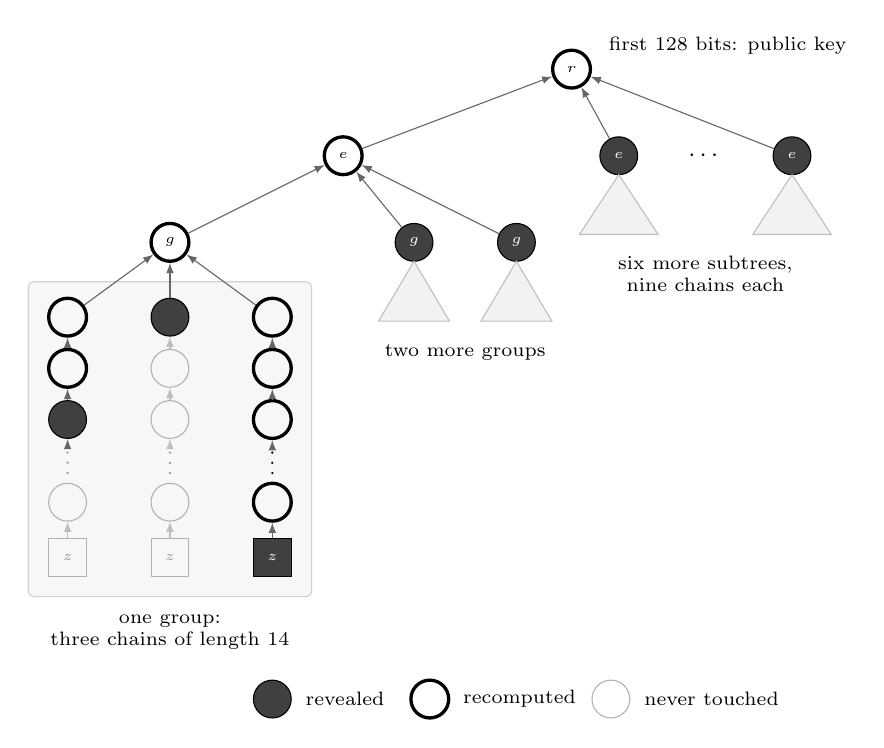
\begin{tikzpicture}[x=1cm,y=1cm,
  v/.style={circle,draw,minimum size=4.8mm,inner sep=0pt,font=\tiny},
  sq/.style={rectangle,draw,minimum size=4.8mm,inner sep=0pt,font=\tiny},
  rev/.style={fill=black!75,text=white},
  hid/.style={draw=black!30,text=black!40},
  ev/.style={very thick},
  a/.style={-{Latex[length=1.3mm]},draw=black!60},
  ah/.style={-{Latex[length=1.3mm]},draw=black!25},
  note/.style={font=\scriptsize,align=center}]

\draw[rounded corners=2pt,draw=black!18,fill=black!3] (-0.5,-0.5) rectangle (3.1,3.5);

% chain 1: a value revealed in the middle of the chain
\node[sq,hid] (z1) at (0,0) {$z$};
\node[v,hid] (p1) at (0,0.7) {};
\fill[black!40] (0,1.07) circle (0.45pt) (0,1.2) circle (0.45pt) (0,1.33) circle (0.45pt);
\node[v,rev] (q1) at (0,1.75) {};
\node[v,ev] (s1) at (0,2.4) {};
\node[v,ev] (t1) at (0,3.05) {};
\draw[ah] (z1)--(p1); \draw[a] (0,1.45)--(q1); \draw[a] (q1)--(s1); \draw[a] (s1)--(t1);

% chain 2: the chain end is revealed
\node[sq,hid] (z2) at (1.3,0) {$z$};
\node[v,hid] (p2) at (1.3,0.7) {};
\fill[black!40] (1.3,1.07) circle (0.45pt) (1.3,1.2) circle (0.45pt) (1.3,1.33) circle (0.45pt);
\node[v,hid] (q2) at (1.3,1.75) {};
\node[v,hid] (s2) at (1.3,2.4) {};
\node[v,rev] (t2) at (1.3,3.05) {};
\draw[ah] (z2)--(p2); \draw[ah] (1.3,1.45)--(q2); \draw[ah] (q2)--(s2); \draw[ah] (s2)--(t2);

% chain 3: the source itself is revealed
\node[sq,rev] (z3) at (2.6,0) {$z$};
\node[v,ev] (p3) at (2.6,0.7) {};
\fill (2.6,1.07) circle (0.45pt) (2.6,1.2) circle (0.45pt) (2.6,1.33) circle (0.45pt);
\node[v,ev] (q3) at (2.6,1.75) {};
\node[v,ev] (s3) at (2.6,2.4) {};
\node[v,ev] (t3) at (2.6,3.05) {};
\draw[a] (z3)--(p3); \draw[a] (2.6,1.45)--(q3); \draw[a] (q3)--(s3); \draw[a] (s3)--(t3);

\node[note] at (1.3,-0.95) {one group:\\three chains of length 14};

% grouping level 1
\node[v,ev] (g1) at (1.3,4.0) {$g$};
\draw[a] (t1)--(g1); \draw[a] (t2)--(g1); \draw[a] (t3)--(g1);
\node[v,rev] (g2) at (4.4,4.0) {$g$};
\node[v,rev] (g3) at (5.7,4.0) {$g$};
\draw[fill=black!5,draw=black!25] (4.4,3.76)--(3.95,3.0)--(4.85,3.0)--cycle;
\draw[fill=black!5,draw=black!25] (5.7,3.76)--(5.25,3.0)--(6.15,3.0)--cycle;
\node[note] at (5.05,2.6) {two more groups};

% grouping level 2
\node[v,ev] (e1) at (3.5,5.1) {$e$};
\draw[a] (g1)--(e1); \draw[a] (g2)--(e1); \draw[a] (g3)--(e1);
\node[v,rev] (e2) at (7.0,5.1) {$e$};
\node[font=\small] at (8.1,5.1) {$\cdots$};
\node[v,rev] (e7) at (9.2,5.1) {$e$};
\draw[fill=black!5,draw=black!25] (7.0,4.86)--(6.5,4.1)--(7.5,4.1)--cycle;
\draw[fill=black!5,draw=black!25] (9.2,4.86)--(8.7,4.1)--(9.7,4.1)--cycle;
\node[note] at (8.1,3.6) {six more subtrees,\\nine chains each};

% root
\node[v,ev] (r) at (6.4,6.2) {$r$};
\draw[a] (e1)--(r); \draw[a] (e2)--(r); \draw[a] (e7)--(r);
\node[note,anchor=west] at (6.75,6.5) {first 128 bits: public key};

% legend
\node[v,rev] at (2.6,-1.8) {}; \node[note,anchor=west] at (2.9,-1.8) {revealed};
\node[v,ev] at (4.6,-1.8) {}; \node[note,anchor=west] at (4.9,-1.8) {recomputed};
\node[v,hid] at (6.9,-1.8) {}; \node[note,anchor=west] at (7.2,-1.8) {never touched};
\end{tikzpicture}
\caption{The computation and one signature. Chain values, group digests $g$ and subtree digests $e$ hold 128 bits each. The revealed values form a cut: exactly one on every path from a source to the root. A signature may reveal a value low on a chain, a chain end, a source, or a digest standing for a whole subtree. The verifier recomputes everything above the cut, here 105 units' worth, and compares the first 128 bits of the root with the public key.}
\label{fig:scheme}
\end{figure}

\paragraph{Disclosure sets.}
A \emph{cut} is a set $A$ of nodes other than the root that meets every path from a source to the root exactly once. Reconstruction at $A$ evaluates the hash nodes strictly above $A$; write $\mathrm{cost}(A)$ for their total cost. Let
\[
D=\{A\ \text{a cut}:\ \mathrm{cost}(A)=105\}.
\]
A direct count gives $|D|=43124494150885380367098178978085896>2^{115}$, while the number of cuts of cost 104 is below $2^{115}$. Fix an injection $\pi:\{0,\dots,M-1\}\to D$, and let $A_i=\pi(i)$. The root is not revealed, and every source-to-root path meets $A_i$, so the conditions of Section~\ref{sec:model} hold.

\paragraph{Costs.}
Key generation evaluates every node: $63\cdot14$ chain hashes, 21 and 7 grouping hashes, and the root, for
\[
63\cdot14+21+7+2=912\le1024\ \text{units}.
\]
A cut of cost 105 has between 15 and 41 nodes, so a signature reveals between 2176 and 5248 bits and has at most 5504 bits. Every signature verifies in
\[
1+105=106\ \text{units},
\]
one unit for the index and 105 for reconstruction.

\paragraph{Why equal cost.}
If one cut evaluates a strict subset of the nodes evaluated by another, it costs strictly less, because every hash node costs at least one unit. Two distinct cuts of equal cost are therefore incomparable: each one reveals a node that the other evaluates. This is what the security proof uses, and it is the only property of $D$ that it needs.

\subsection{Distance from the lower bound}

Theorem~\ref{thm:main} leaves a gap between 25 and 106 units. The following heuristic suggests that most of this gap cannot be closed by schemes of the usual kind. It is not a proof, and the gap remains open: it rests on an assumption about how forgeries arise that the model of Section~\ref{sec:model} does not impose. Suppose that forging at index $j$ from a signature at index $i\ne j$ always requires the output of a hash node revealed at $i$ and evaluated at $j$, that is, $A_i\cap E_j\ne\emptyset$, while $A_i\cap E_i=\emptyset$. Bollob\'as's set-pair inequality gives $\sum_i\binom{|A_i|+|E_i|}{|A_i|}^{-1}\le1$. A signature reveals at most 41 hash values of 128 bits, so $2^{115}$ disclosure sets force $|E_i|\ge93$ for some $i$, since $\binom{41+92}{41}<2^{115}$. The scheme above evaluates 104 hash nodes and costs two units more, because of its root.

Among all forests of this shape, chains of one length under up to four levels of grouping, with branching factors up to 41 and optional chains of digests above the grouping nodes, an exhaustive computer search within the key-generation budget found nothing below 106 units. Flat variants are slightly worse: 41 chains of length 16 whose ends are hashed together, with the digits of the revealed positions summing to 96, give a Winternitz signature with a constant-sum encoding that verifies in 108 units. Beating the barrier above requires constraints spread over several revealed values, which is exactly the situation the attack of Theorem~\ref{thm:main} exploits.

\subsection{Security}

\begin{theorem}\label{thm:scheme}
Let an attacker's experiment with the scheme cost at most $B$ on every execution path, where $B\le2^{233}$. Then
\[
\Pr[\mathrm{Forge}]\le\frac{B-913}{2^{127}}.
\]
In particular the scheme satisfies~\eqref{eq:security} for every $B$.
\end{theorem}

The final claim follows because an attacker with $B>2^{233}$ satisfies~\eqref{eq:security} trivially.

\paragraph{Key generation.}
Write $x_v$ for the value that key generation computes at the node $v$, and $\pk$ for the public key. Each hash node $v$ is queried once, at the point $P_v$ formed by its label and the values of its children (its source for the first node of a chain). The labels are distinct, so all these queries are fresh: the sources and the hash outputs are independent and uniform.

We classify the remaining queries by who makes them. The signer only queries the message encoding. The attacker queries in both of its stages, and the verifier queries while checking the claimed forgery.

\paragraph{Hidden points.}
Until signing returns a signature, and throughout if signing fails, every key-generation point is \emph{hidden}. If signing returns a signature at index $i$, then from that moment $P_v$ is hidden exactly when $v$ lies at or below the cut $A_i$, that is, when $v\in A_i$ or no path from $v$ to the root meets $A_i$ above $v$. The inputs of those points lie strictly below the revealed values. All other key-generation points become exposed.

\paragraph{Events.}
We consider the following events, each concerning a query made by the attacker or by the verifier.
\begin{description}
\item[$E_{\mathrm{hid}}$:] the query is at a point that is hidden at the time of the query.
\item[$E_{\mathrm{spr}}$:] the query is the first one at a point that is not a key-generation point, its label is that of a node $v$, and its answer begins with $x_v$; or its label is that of the root and its answer begins with $\pk$.
\item[$E_{\mathrm{idx}}$:] signing succeeds at the encoding input $u_1=m_1\Vert\eta_1$ with index $i$, and the query is at an encoding input $u\ne u_1$ whose index is $i$.
\end{description}

\begin{lemma}\label{lem:scheme-events}
Every successful forgery causes $E_{\mathrm{hid}}$, $E_{\mathrm{spr}}$ or $E_{\mathrm{idx}}$.
\end{lemma}

\begin{proof}
Let the verifier accept $(m_2,\eta_2,x')$ and let $j$ be the index of $m_2\Vert\eta_2$. The verifier computes a value $x'_v$ at every node $v$ evaluated at $A_j$, takes the supplied values at the nodes of $A_j$, and its root query returns an output beginning with $\pk$. If the root input differs from $e_1\Vert\cdots\Vert e_7$, the first query at that point is not at a key-generation point and causes $E_{\mathrm{spr}}$. Assume from now on that the root input agrees, so $x'_{e_l}=x_{e_l}$ for every $l$.

We use the following walk. Let $v$ be a node evaluated at $A_j$, and let $v=v_0,v_1,\dots,v_m$ be the path from $v$ to the child of the root, so that $x'_{v_m}=x_{v_m}$. Let $t^*$ be the least index with $x'_{v_{t^*}}=x_{v_{t^*}}$. If $t^*>0$, the verifier's query at the hash node of $v_{t^*}$ has an input different from the honest one, because $x'_{v_{t^*-1}}\ne x_{v_{t^*-1}}$, and an answer beginning with $x_{v_{t^*}}$; that point is not a key-generation point, so its first query causes $E_{\mathrm{spr}}$. If $t^*=0$, the verifier's query at the hash node of $v$ has an answer beginning with $x_v$; either its input differs from the honest one, which causes $E_{\mathrm{spr}}$ as before, or the query is at the key-generation point $P_v$.

\emph{Signing failed.} Every key-generation point is hidden. Since $\mathrm{cost}(A_j)=105$, some node $v\ne r$ is evaluated at $A_j$. The walk from $v$ gives $E_{\mathrm{spr}}$, or a query at the hidden point $P_v$, which causes $E_{\mathrm{hid}}$.

\emph{Signing succeeded at index $j\ne i$.} The cuts $A_i$ and $A_j$ are distinct of equal cost, so some node $v$ is revealed at $A_i$ and evaluated at $A_j$. The walk from $v$ gives $E_{\mathrm{spr}}$, or a query at $P_v$, which is hidden because $v$ lies on the cut $A_i$; that causes $E_{\mathrm{hid}}$.

\emph{Signing succeeded at index $j=i$, with $m_2\Vert\eta_2\ne m_1\Vert\eta_1$.} The verifier's encoding query at $m_2\Vert\eta_2$ causes $E_{\mathrm{idx}}$.

\emph{Signing succeeded at index $j=i$, with $m_2\Vert\eta_2=m_1\Vert\eta_1$.} The forgery differs from the signature and both reveal the values of $A_i$, so $x'_v\ne x_v$ for some $v\in A_i$. The parent of $v$ is evaluated, and the walk started there causes $E_{\mathrm{spr}}$.
\end{proof}

\begin{lemma}\label{lem:scheme-probabilities}
Let $N_{\mathrm{h}}$ and $N_{\mathrm{e}}$ be the numbers of queries made by the attacker and the verifier with a node label, and with the encoding label. Then
\[
\Pr[E_{\mathrm{spr}}]\le\frac{\mathbb E[N_{\mathrm{h}}]}{2^{128}},\qquad
\Pr[E_{\mathrm{hid}}]\le\frac{\mathbb E[N_{\mathrm{h}}]}{2^{128}},\qquad
\Pr[E_{\mathrm{idx}}]\le\frac{2\,\mathbb E[N_{\mathrm{e}}]}{2^{128}}.
\]
\end{lemma}

\begin{proof}
\emph{The event $E_{\mathrm{spr}}$.} The first query at a point that is not a key-generation point receives a fresh uniform 256-bit answer. The value it must begin with, $x_v$ or $\pk$, is fixed at key generation. Each such query therefore causes $E_{\mathrm{spr}}$ with probability $2^{-128}$, and a union bound over the queries gives the claim.

\emph{The event $E_{\mathrm{hid}}$.} Consider the modified experiment in which every query at a point that is hidden at the time of the query receives a fresh uniform answer. The two experiments agree until the first query at a hidden point, so the probability of $E_{\mathrm{hid}}$ is the same in both. In the modified experiment the hidden inputs are independent of everything else. Before signing, the transcript depends on key generation only through $\pk$, which is independent of the other values. The index chosen by signing depends only on encoding answers. After a signature at index $i$, the transcript depends on key generation through the values at and above the cut $A_i$, while the input of a hidden point is a function of the sources and of the hash outputs strictly below $A_i$. The input of a hidden point on a chain is uniform on 128 bits, and the input of a hidden grouping node or of the root is uniform on 384 or 896 bits. Hence each query hits the hidden point of its label with probability at most $2^{-128}$, and a union bound over the queries gives the claim.

\emph{The event $E_{\mathrm{idx}}$.} Let $u$ be a query by the attacker or the verifier at an encoding input $u\ne u_1$. If $u$ was queried before, the first query at $u$ was made by the attacker or by the signer. A signer query at $u\ne u_1$ returned an invalid index, which is never $i$. We may therefore charge the event to the first query at $u$ by the attacker or the verifier, which is fresh.

If this first query happens after signing, its index equals $i$ with probability $2^{-128}$.

If it happens before signing, its index $j$ is valid with probability $2^{-13}$. Given the transcript up to that point, signing ends with index $j$ only if one of its trials returns $j$. A trial at a fresh input does so with probability $2^{-128}$. The expected number of trials is at most $2^{13}+\mathbb E[F]$, where $F$ counts the trials at inputs queried earlier by the attacker. A trial at such an input $u'\ne u$ returns $j$ only if $u'$ and $u$ have equal indices, which happens with probability $2^{-128}$ over the answer at $u$. Each trial lands on one of the at most $B$ earlier attacker inputs with probability at most $B/(2^{256}-L)$. Altogether this first query causes $E_{\mathrm{idx}}$ with probability at most
\[
2^{-13}\bigl(2^{13}+LB\,2^{-255}\bigr)2^{-128}+LB\,2^{-255}\cdot2^{-128}\le2\cdot2^{-128},
\]
using $LB\le2^{21}\cdot2^{233}=2^{254}$. A union bound over the queries gives the claim.
\end{proof}

\begin{proof}[Proof of Theorem~\ref{thm:scheme}]
By the two lemmas,
\[
\Pr[\mathrm{Forge}]\le\frac{2\,\mathbb E[N_{\mathrm{h}}]+2\,\mathbb E[N_{\mathrm{e}}]}{2^{128}}=\frac{\mathbb E[N_{\mathrm{h}}+N_{\mathrm{e}}]}{2^{127}}.
\]
Every query costs at least one unit. On every path, key generation costs 912 units and signing at least one more, so the attacker and the verifier make at most $B-913$ queries. This proves the bound. For $B\le2^{233}$ it gives $\Pr[\mathrm{Forge}]<B/2^{127}$, and for larger $B$ the requirement~\eqref{eq:security} holds because its right-hand side exceeds one.
\end{proof}

\appendix

\section{Entropy facts and a repetition estimate}\label{sec:elementary}

We give the entropy identities and the bound for repeated attempts used in the proof. All distributions below have finite support, and sums omit terms of zero probability. Logarithms are base two unless written $\ln$.

\paragraph{Nonnegativity of relative entropy.}
The function $u-1-\ln u$ on $u>0$ has derivative $1-1/u$ and minimum zero at $u=1$. Hence $-\ln u\ge1-u$. For distributions $P,Q$ with $P(x)>0$ whenever $Q(x)>0$, apply this inequality with $u=P(x)/Q(x)$ and average under $Q$:
\[
(\ln2)\KL(Q\Vert P)
\ge\sum_{x:Q(x)>0}(Q(x)-P(x))\ge0.
\]
The last inequality holds because $Q$ sums to one on this set, whereas $P$ sums to at most one. If $P(x)=0<Q(x)$ anywhere, the relative entropy is infinite and the conclusion still holds.

\paragraph{The entropy chain rule.}
For finite random variables $A,B$ with joint distribution $P$, factor their joint probability as $P(a,b)=P_A(a)P(b\mid a)$, where $P_A$ is the distribution of $A$. Taking negative logarithms and averaging gives
\[
\Ent(A,B)=\Ent(A)+\Ent(B\mid A)=\Ent(B)+\Ent(A\mid B).
\]
The first equality uses $-\log P(a,b)=-\log P_A(a)-\log P(b\mid a)$; exchanging $A$ and $B$ gives the second. Repeating this identity expresses the entropy of a record as the entropy of its first entry plus the conditional entropies of successive entries. A fixed entry contributes zero. A variable uniform on a set of size $m$ has entropy $\sum_{k=1}^m(1/m)\log m=\log m$.

\paragraph{Conditioning and maximum entropy.}
Expanding the definitions gives
\[
\Ent(A\mid B)-\Ent(A\mid B,C)
=\mathbb E_{b,c}\KL(P_{A\mid b,c}\Vert P_{A\mid b})\ge0.
\]
The expectation is over the joint distribution of $B,C$. Thus an additional conditioning variable cannot increase conditional entropy. If a random variable $A$ takes values in a set of size $m$, compare its distribution $P_A$ with the uniform distribution $U$ on that set:
\[
0\le\KL(P_A\Vert U)=\log m-\Ent(A).
\]
In particular, a variable with at most $2^t$ possible values has entropy at most $t$.

\paragraph{Success after repeated attempts.}
When independent attempts each succeed with probability $p$, all $q$ fail with probability $(1-p)^q$. The following inequality bounds this failure probability using $-\ln p$.

\begin{lemma}[Repetition estimate]\label{lem:repetition}
For every integer $q\ge3$ and every $0<p\le1$,
\[
(1-p)^q\le\frac{-\ln p}{\ln q+\ln\ln q+1}.
\]
\end{lemma}

\begin{proof}
For $p=1$, both sides are zero. Otherwise, put $u=-\ln p>0$. It suffices to prove $G(u)\ge\ln q+\ln\ln q+1$ for
\[
G(u)=\frac{u}{(1-e^{-u})^q}.
\]
This function tends to infinity as $u$ approaches either endpoint of $(0,\infty)$. Its derivative has the sign of $e^u-1-qu$. This last function is strictly convex, equals zero at zero, has negative derivative there, and tends to infinity. It therefore has exactly one positive zero $u_*$, where $G$ attains its minimum and
\[
e^{u_*}=1+qu_*.
\]

For $q\ge3$, we have $\ln q>1$. Evaluating $e^u-1-qu$ at $u=\ln q$ gives a negative value, so $u_*>\ln q$. Hence
\[
u_*=\ln(1+qu_*)>\ln q+\ln u_*>\ln q+\ln\ln q.
\]
At the minimum, the binomial theorem gives
\[
G(u_*)=u_*\left(1+\frac1{qu_*}\right)^q
\ge u_*+1>\ln q+\ln\ln q+1.
\]
Since $G(u)\ge G(u_*)$, the result follows. For completeness, $\ln3>1$ follows from $e<3$: in the series $e=\sum_{k\ge0}1/k!$, the terms for $k\ge2$ sum to less than $\sum_{k\ge2}2^{-(k-1)}=1$.
\end{proof}

\section{Exact numerical bounds}\label{sec:numerical}

This appendix verifies the bounds on $\beta_{22}$, the construction budget, the forgery probability, and the total cost. Each numerical comparison uses exact rational arithmetic.

\paragraph{The counting factor.}
Substituting $S_*=5257$, $a=22$, and $d=123$ into~\eqref{eq:beta} gives
\[
\beta_{22}(123)
=\frac{123^{22}\prod_{k=1}^{22}(110397+5380k)}
{5380^{22}\prod_{k=1}^{22}(115654+123k)}.
\]
Cross multiplication gives $103<2^{115}\beta_{22}(123)<104$, so in particular $M\beta_{22}(123)>100$. For the monotonicity used in~\eqref{eq:rank-bound}, write
\[
\frac{\beta_{22}(d)}{d^{22}}
=\prod_{k=1}^{22}\frac{21S_* /(S_*+d)+k}{22S_*+kd}.
\]
Each numerator is positive and decreasing, and each denominator is positive and increasing. The product is therefore decreasing for $d>0$.

\paragraph{The construction budget.}
The exponential series gives $e>1+1+1/2+1/6=8/3$. Also,
\[
\ln2=2\int_0^{1/3}\frac{1}{1-t^2}\,\mathrm{d}t
>2\int_0^{1/3}(1+t^2)\,\mathrm{d}t=\frac{56}{81}.
\]
For $q=5\cdot2^{113}$, these bounds imply
\[
e q\ln q>
\frac83\cdot5\cdot2^{113}\cdot113\cdot\frac{56}{81}
=\frac{253120}{243}\,2^{113}
>2^{123}.
\]
Thus $\log(e q\ln q)>123$, as required.

\paragraph{A rational bound for nonce selection.}
For the probabilities $\omega_\ell$ defined in Section~\ref{sec:attack}, put $\lambda=T/N=3/128$. We will use a polynomial lower bound on the exponential. Define
\[
P_k(y)=\sum_{h=0}^k\frac{(-y)^h}{h!}
\qquad(k=6,7).
\]
For $y\ge0$, Taylor's theorem gives $P_7(y)\le e^{-y}\le P_6(y)$. Hence $P_7'(y)=-P_6(y)<0$. Since
\[
P_7(100\lambda)=P_7(75/32)=\frac{300676096241}{3848290697216}>0,
\]
all the values $P_7(\ell \lambda)$ for $1\le\ell\le100$ are positive.

Integrating the derivative of $(1-y/N)^T$ gives
\[
\omega_\ell
=\lambda\int_{\ell-1}^{\ell}(1-y/N)^{T-1}\,\mathrm{d}y
\ge \lambda(1-\ell/N)^{T-1}.
\]
For $0\le u<1$,
\[
-\ln(1-u)=u+\int_0^u\frac{t}{1-t}\,\mathrm{d}t
\le u+\frac{u^2}{1-u}.
\]
Take $u=\ell/N<1/2$. Since $\ell\le100$ and $T<N/32$, we obtain
\[
(T-1)\ln(1-u)\ge-\ell \lambda-\frac{Tu^2}{1-u},
\qquad
\frac{Tu^2}{1-u}<\frac{625}{N}.
\]
Using $e^{-y}\ge1-y$ and $e^{-\ell \lambda}\le1$ now gives
\begin{equation}\label{eq:omega-certificate}
\omega_\ell
\ge \lambda e^{-\ell \lambda}-\frac{625\lambda}{N}
> \lambda P_7(\ell \lambda)-2^{-120}.
\end{equation}
The final inequality uses $625\lambda<20<256$ and $N=2^{128}$.

\paragraph{An exact bound for the success probability.}
The formula for $b_\ell$ in~\eqref{eq:rank-success} contains $z_\ell^{1/22}$. Round this root upward to a multiple of $2^{-32}$. More precisely, for $2\le\ell\le100$, define
\[
z_\ell=\frac{512(\ell-1)}{51100},
\qquad
k_\ell=\min\left\{k\in\{0,\ldots,2^{32}\}:
51100k^{22}\ge512(\ell-1)2^{704}\right\}.
\]
The minimum exists because $z_\ell<1$, so $k=2^{32}$ satisfies the inequality. Its definition gives $k_\ell/2^{32}\ge z_\ell^{1/22}$. Set
\[
\underline b_1=1,\qquad
\underline b_\ell=\frac{511}{512}
\left(1-\frac{22k_\ell}{21\cdot2^{32}}+\frac{z_\ell}{21}\right).
\]
The coefficient of the root in $b_\ell$ is negative, so $\underline b_\ell\le b_\ell$.

Each $k_\ell$ is determined by integer comparisons: its defining inequality holds at $k_\ell$ and fails at $k_\ell-1$. Substituting these integers and adding the rational terms gives
\[
\lambda\sum_{\ell=1}^{100}\underline b_\ell P_7(\ell \lambda)
=\frac{43420993900138087655153856906939}
{776435992639790508416730713292800}
>\frac{559}{10000}.
\]
Multiply~\eqref{eq:omega-certificate} by $b_\ell$ and sum. Since $P_7(\ell \lambda)>0$, $\underline b_\ell\le b_\ell$, and $0\le b_\ell\le1$, we obtain
\[
\begin{aligned}
(1-\delta)\sum_{\ell=1}^{100}\omega_\ell b_\ell
&>(1-2^{-256})
\left(\frac{559}{10000}-100\cdot2^{-120}\right)\\
&>\frac{11}{200}.
\end{aligned}
\]
The last comparison follows by cross multiplication.

\paragraph{The total cost.}
Substituting the attack's budgets gives
\[
B=1024+2^{21}+3\cdot2^{121}+(5\cdot2^{113}+2)\cdot23+2.
\]
Direct comparison of these integers shows
\[
\frac{B}{2^{127}}<\frac{27}{500}<\frac{11}{200},
\]
completing the numerical bounds used in the theorem.

\end{document}
